\chapter{Implementácia}
\label{chap:implementation}

V~tejto kapitole predstavíme triedy a popíšeme implementačné detaily jednotlivých častí algoritmu.

Budeme sa venovať základným triedam, riešeniam elementárnych vecí, detailom spracovania obrazu, rozpoznávaniu ruky a gesta. Podrobne si popíšeme implementáciu neurónových sietí.

Spomenieme aj niektoré problémy a ich riešenia a možnosti paralelizácie.

\bigskip

\section{Neurónové siete}

Naša implementácia neurónových sietí kopíruje vrstvový model. Základnou jednotkou je spojitý perceptrón, skupinu perceptrónov zastrešuje vrstva a skupinu vrstiev neurónová sieť. 

Ku každej z~týchto úrovní máme všeobecnú triedu a rôzne implementácie. Na obrázku \ref{fig:nnclsdiag} je class diagram nášho riešenia.

\begin{figure}[htp]
    \centering
    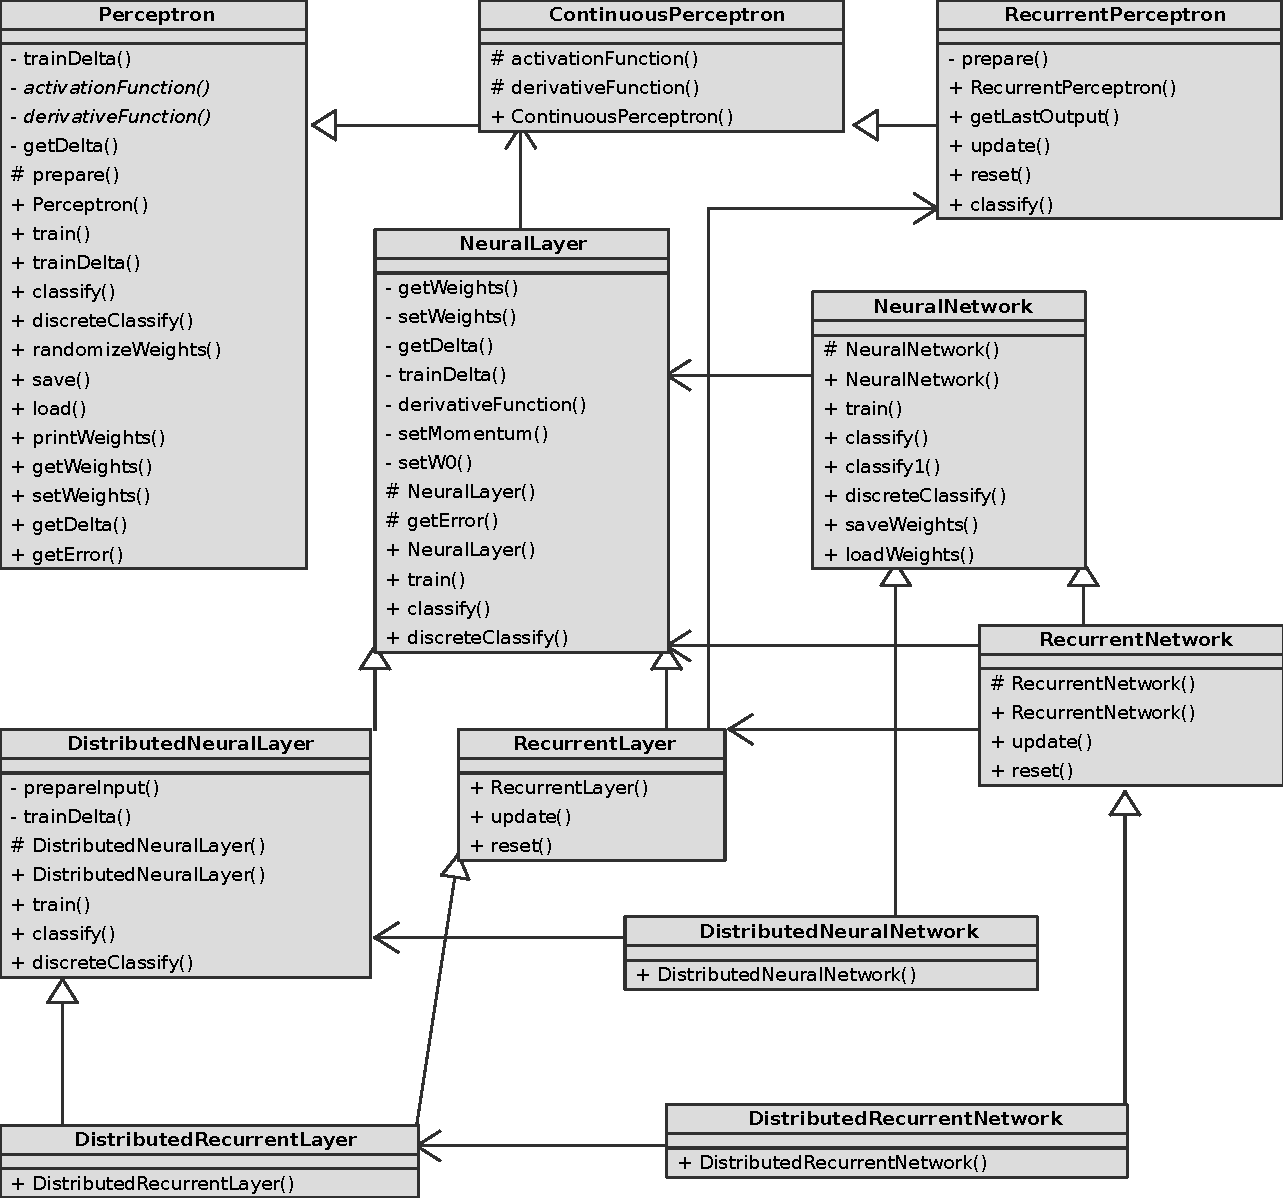
\includegraphics[width=\textwidth]{images/nn_class_diagram}
    \caption{Neurónové siete - Class diagram}
    \label{fig:nnclsdiag}
\end{figure}

\subsection{Perceptron}
\label{sect:perceptron}
\textit{Perceptron} je abstraktná trieda, ktorá zovšeobecňuje rôzne typy perceptrónov, ktoré sa líšia rôznymi aktivačnými funkciami.

Obsahuje trénovací algoritmus pre perceptróny, ale aj podporu algoritmu \textit{backpropagation} a klasifikačný algoritmus. Okrem toho obsahuje užitočné funkcie na randomizáciu váh, ukladanie a načítanie váh.

\textit{Perceptron} pri volaní metód, ktoré majú ako parameter vstup siete si perceptrón sám pridá \textit{bias}\footnote{kapitola \ref{chap:perceptron}}, takže ho nie je nutné pridávať k~vstupu.

Možnosť vytvorenia rôznych typov perceptrónov zabezpečujú abstraktné metódy 
\begin{itemize}
\item \method{float activationFunction(const vector<float>* input)},
\item \method{float derivativeFunction(float x)},
\end{itemize}
ktoré treba v~potomkovi definovať.

\subsubsection{Dôležité metódy}
\begin{itemize}
\item \method{void train(vector<float> input,int target)}
\\Jednoduché trénovanie perceptrónov.
\\ \underline{Vstup:} \textit{input} - vstup siete, \textit{target} - požadovaný výstup 
\item \method{ void trainDelta(vector<float> input, float delta)}
\\Delta trénovanie pre \textit{backpropagation} algoritmus.
\\ \underline{Vstup:} \textit{input} - vstup siete, \textit{delta} $=\delta$ z~učiaceho pravidla: $\Delta w_i = \alpha\delta x_i$\footnote{používame mierne inú notáciu ako je v~\cite{haykin1999neural}} \cite[s. 74]{haykin1999neural}
%\\ \underline{Výstup:} \textit{void}
\item \method{ float classify(vector<float> input)}
\\Klasifikačný algoritmus.
\\ \underline{Vstup:} \textit{input} - vstup siete
\\ \underline{Výstup:} reálne číslo z~intervalu $(0,1)$ - výstup siete.
\item \method{void prepare(vector<float>* input);}
\\Predpríprava vstupu pre spracovanie v~perceptróne - pridáva \textit{bias}.

Túto metódu treba volať tam, kde metóda dostáva užívateľský vstup (bez \textit{biasu}).
\\ \underline{Vstup:} \textit{*input} - pointer vstup siete
\\ \underline{Výstup:} metóda upraví priamo vektor, ktorý jej bol daný ako vstup.
\end{itemize}

\subsection{ContinuousPerceptron}
Trieda \textit{ContinuousPerceptron} je implementácia spojitého perceptrónu. Dedí od triedy \textit{Perceptron} 
Definuje aktivačnú funkciu
$$f(x)=\frac{1}{1+e^{-x}} $$
a jej deriváciu
$$f'(x)=\frac{e^x}{(e^x+1)^2} $$

\subsection{RecurrentPerceptron}
Trieda \textit{RecurrentPerceptron} rozširuje triedu \textit{ContinuousPerceptron} o~rekurentný vstup a metódy na manipulovanie s~ním -- \method{void update()} a \method{void reset()} na update a reset rekurentného vstupu.

\subsection{NeuralLayer}
\textit{NeuralLayer} je trieda, ktorá zoskupuje spojité perceptróny do vrstvy. Umožňuje trénovanie na viacrozmerné výstupy a podporuje \textit{backpropagation} algoritmus. 

Táto trieda poskytuje základnú implementáciu -- predkladá celý vstup každému neurónu. Je zároveň základnou triedou pre vrstvy neurónov, od ktorej potom dedia iné typy vrstiev. Zmena vlastností triedy sa deje v~konštruktore, kde je možné určiť typy jednotlivých neurónov a ich parametre.

\subsubsection{Dôležité metódy}
\begin{itemize}
\item \method{float train(vector<float> input, vector<int> target)}
\\Jednoduché trénovanie jednotlivých perceptrónov.
\\ \underline{Vstup:} \textit{input} - vstup siete, \textit{target} - požadované výstupy 
\\ \underline{Výstup:} chyba na danom vstupe.
\item \method{void trainDelta(vector<float> input,vector<float> delta)}
\\Delta trénovanie pre \textit{backpropagation} algoritmus.
\\ \underline{Vstup:} \textit{input} - vstup siete, \textit{delta} -- delty pre jednotlivé neuróny - podobne ako v~kapitole \ref{sect:perceptron}
%\\ \underline{Výstup:} \textit{void}
\item \method{ vector<float> classify(vector<float> input)}
\\ Klasifikačný algoritmus.
\\ \underline{Vstup:} \textit{input} - vstup siete
\\ \underline{Výstup:} pole čísel z~intervalu $(0,1)$ - výstup siete.
\end{itemize}

\subsection{DistributedNeuralLayer}
Trieda \textit{DistributedNeuralLayer} dedí od triedy \textit{NeuralLayer}. Poskytuje podobnú funkcionalitu ako \textit{NeuralLayer}, ale vstup je rozdelený na $n\times m$ častí a každý neurón má k~dispozícii len jednu časť. 

Okrem konštruktora bolo v~tomto prípade nutné upraviť aj metódy \method{float train(vector<float>,vector<int>)} a \method{vector<float> classify(vector<float>)}, tak, aby trénovanie a klasifikácia prebiehala na príslušnej časti vstupu.

\subsection{RecurrentLayer}
Trieda \textit{RecurrentLayer} dedí od triedy \textit{NeuralLayer}. Namiesto spojitých perceptrónov používa rekurentné. Navyše pridáva metódy \method{void update()} a \method{void reset()}, ktoré umožňujú update a reset rekurentného vstupu neurónov.

\subsection{DistributedRecurrentLayer}
Trieda \textit{DistributedRecurrentLayer} dedí od triedy \textit{RecurrentLayer} a \textit{DistributedRecurrentLayer}. Tu sa ukazuje sila nášho objektovo orientovaného modelu ako aj sila viacnásobného dedenia v~C++. Táto trieda obsahuje len konštruktor, ktorý volá konštruktory rodičovských tried. Prakticky bez námahy vieme takto vytvoriť nový typ siete spojením dvoch existujúcich.

Spojením dvoch typov vrstiev získavame máme nový typ vrstvy, ktorá obsahuje rekurentné neuróny, pričom každý z~nich má k~dispozícii len časť vstupu.

\subsection{NeuralNetwork}
Trieda \textit{NeuralNetwork} zoskupuje vrstvy do viacvrstvovej siete. Implementuje viacvrstvovú sieť s~vrstvami typu \textit{NeuralLayer} a zároveň slúži ako základná trieda pre neurónové siete, od ktorej potom dedia ostatné siete.

Poskytuje implementáciu \textit{backpropagation} algoritmu, ukladanie a načítanie váh do/zo súboru. 

Dediace triedy väčšinou mierne menia architektúru napríklad použitím iného typu vrstvy. Tieto zmeny sa zvyknú robiť v~konštruktore.

\subsubsection{Dôležité metódy}
\begin{itemize}
\item \method{float train(vector<float> input, vector<int> target)}
\\\textit{Backpropagation} algoritmus.
\\ \underline{Vstup:} \textit{input} - vstup siete, \textit{target} - požadované výstupy 
\\ \underline{Výstup:} chyba na danom vstupe.
\item \method{ vector<float> classify(vector<float> input)}
\\ Klasifikačný algoritmus.
\\ \underline{Vstup:} \textit{input} - vstup siete
\\ \underline{Výstup:} pole čísel z~intervalu $(0,1)$ - výstup siete.
\end{itemize}

\subsection{DistributedNeuralNetwork}
Trieda \textit{DistributedNeuralNetwork} dedí z~\textit{NeuralNetwork}. Jedinou zmenou je, že ako spodnú vrstvu používa \textit{DistributedNeuralLayer}.

\subsection{RecurrentNetwork}
Trieda \textit{RecurrentNetwork} je potomkom triedy \textit{NeuralNetwork}. Ako spodnú vrstvu používa \textit{RecurrentLayer}. Okrem toho implementuje metódy \method{update()} a \method{reset()}, ktoré updatujú a resetujú rekurentnú vrstvu.

\subsection{DistributedRecurrentNetwork}
Trieda \textit{DistributedRecurrentNetwork} dedí z~\textit{RecurrentNetwork}. Ako spodnú vrstvu používa \textit{DistributedRecurrentLayer}.

\section{Triedy pre obrázky}

Pre účely aplikácie potrebujeme špecifickú triedu na obrázky, ktorá spĺňa nasledujúce vlastnosti:
\begin{itemize}
\item Rýchly prístup k~jednotlivým pixlom.
\item Vystrihnutie(crop)
\item Škálovanie
\item Maskovanie
\item Floodfill
\end{itemize}
Okrem toho potrebujeme aby obsahovala aj pomocné metódy, ktoré sú potrebné na niektoré algoritmy a testovanie, konverziu do rôznych formátov, ukladanie na disk a~iné.

Trieda \textit{HCImage}, je abstraktná trieda, ktorá implementuje základné veci, ktoré sú nezávislé na type pixlu. Od tejto triedy potom dedia triedy \textit{GrayScaleImage} a \textit{ColorImage}. Tieto implementujú metódy, ktoré sú závislé na type pixlu (odtiene šedej alebo farebný pixel). 

\subsubsection{Vystrihnutie}
Na vystrihnutie slúži metóda \method{copy(QRect r)}, ktorá berie ako parameter obdĺžnik, ktorého obsah potom vráti ako výsledok. 

\subsubsection{Škálovanie}
\label{chap:scale}
Metóda \method{scale(unsigned w, unsigned h)} preškáluje obrázok na novú veľkosť - $w\times h$ pixlov.

Využíva bilineárnu interpoláciu -- vypočíta súradnice nového bodu a pomocou susedných bodov z~pôvodného obrázka vypočíta farbu.

Bilineárna interpolácia má niekoľko výhod. Je stále dosť rýchla, pričom eliminuje kostrbatosť, ktorá môže mať výrazný vplyv pri použití Fourierovej transformácie.

\subsubsection{Maskovanie}

Metóda \method{mask(HCImage *mask, bool invert = false)} aplikuje masku na obrázok. Hodnotu každej farby zníži podľa hodnoty masky v~danom bode.

Maskovanie použijeme na odstránenie nepodstatných častí obrázka, aby neovplyvňovali neurónovú sieť. Využívame bitové operátory na urýchlenie výpočtu. %Každý pixel skombinuje s~pixlom masky. 

\subsubsection{Floodfill selekcia}
Techniku \textit{floodfill selekcie} si môžeme predstaviť ako ,,čarovnú paličku''\footnote{známu z~grafických programov ako je GIMP, či Photoshop}, alebo nástroj na selekciu susedných pixlov s~podobnými farbami. Techniku \textit{floodfill} používame na získanie masky v~metóde \method{getAdaptiveFloodFillSelectionMask(int sx, int sy, int treshold, float originalFactor, float changeFactor)} (Obr. \ref{fig:getAdaptiveFloodFillSelectionMask}). Metóda berie nekoľko parametrov -- pozíciu bodu z~ktorého má floodfill začať, hranicu podobnosti farieb, vplyv originálnej farby a zmeny. Referenčná farba sa získa ako priemer začiatočného bodu a jeho okolitých bodov. 

Metóda vráti obrázok, ktorý sa dá použiť ako maska, ktorá odstráni\footnote{začierni} pixle, ktoré neboli vybraté pomocou techniky \textit{floodfill}.

Algoritmus funguje ako prehľadávanie do šírky, pričom do susedného pixlu pôjde len v~prípade, že ich rozdiel je menší ako hranica. V~prípade farebného obrázka sa tento rozdiel počíta po zložkách a menší musí byť každý z~nich. Pri prejdení do nasledujúceho pixlu sa upraví referenčná farba podľa nasledujúceho vzorca: $refcolor = reference \cdot originalFactor + (refcolor\cdot changeFactor+color \cdot (1-changeFactor)) \cdot (1-originalFactor)$, kde $reference$ je začiatočná referenčná farba, $refcolor$ je aktuálna referenčná farba a $color$ je farba pixlu.

\begin{figure}[htp]
\begin{lstlisting}
template <class T>
HCImage<T>* HCImage<T>::getAdaptiveFloodFillSelectionMask(unsigned sx, unsigned sy, int treshold, float originalFactor, float changeFactor)
{
  T reference = getAverageColor(sx,sy);
  ImageBuffer b;
  b.resize(width()*height(),0);
  queue<pair<pair<unsigned,unsigned>,T> > f;
  f.push(make_pair(make_pair(sx,sy),reference));
  while(!f.empty())
  {
      unsigned x = f.front().first.first;
      unsigned y = f.front().first.second;
      T refcolor = f.front().second;
      f.pop();
      if(x>=width()) continue;
      if(y>=height()) continue;

      T color = pixel(x,y);
      if(!similar(refcolor,color,treshold) || b[x+y*w]!=T(0)) continue;
      b[x+y*w]=0xffffffff;
      refcolor = reference*originalFactor + (refcolor*changeFactor+color*(1-changeFactor))*(1-originalFactor);

      f.push(make_pair(make_pair(x+1,y),refcolor));
      f.push(make_pair(make_pair(x-1,y),refcolor));
      f.push(make_pair(make_pair(x,y+1),refcolor));
      f.push(make_pair(make_pair(x,y-1),refcolor));
  }
  HCImage<T> * maskImage = create(b,width(),height());
  return maskImage;
}\end{lstlisting}
\caption{Zdrojový kód funkcie HCImage<T>::getAdaptiveFloodFillSelectionMask()}
\label{fig:getAdaptiveFloodFillSelectionMask}
\end{figure}

\section{Získanie obrazu z~webkamery}
Na získanie obrazu z~webkamery používam triedu, ktorá pochádza z~programu \textit{Kapture} \cite{kapture} a ktorú sme upravili pre potreby využitia v~našej aplikácii. Program je šírený pod GNU GPL licenciou.

Webkamera vracia obraz vo formáte MJPEG(Motion JPEG), teda postupnosť obrázkov vo formáte JPEG. Úlohou našej triedy je vždy keď je buffer pripravený, zobrať pretransformovať obrázok do niektorej z~tried na obrázky. JPEG kóduje farby vo formáte YUV, tieto teda musíme pretransformovať do RGB. V~prípade čiernobieleho obrázka iba zoberieme zložku Y.

\section{Spracovanie obrazu - Trieda ImageProcessor}
\label{chap:imageprocess}
Trieda \textit{ImageProcessor} má na starosti predspracovanie obrazu z~webkamery, jeho segmentáciu a posunutie na ďalšie spracovanie triede \textit{HandRecognizer}. \textit{ImageProcessor} využíva vlákna na paralelizáciu úloh a jeho práca je rozdelená do niekoľkých krokov, ktoré nemôžu byť vykonané paralelne. Hlavná metóda je metóda \method{processImage (const GrayScaleImage \&image, const ColorImage \&colorimg)}, ktorá spravuje vlákna a spúšťa jednotlivé kroky. 

Spúšťanie vláken je realizované pomocou funkcie \method{QtConcurrent::run(Function function, ...)} z~knižnice \textit{Qt}, ktorá umožňuje spustiť funkciu s~danými parametrami v~novom vlákne. Jednotlivé metódy sú upravené tak, aby vedeli upravovať aj len určitú časť obrázka. Spúšťajú sa v~rôznych vláknach s~rôznymi časťami obrázka. %Kritické časti sme ohraničili mutexami.

\subsection{Krok 1: Príprava}
Príprava spočíva vo vytvorení rozdielového obrázka. Pamätáme si pôvodný obrázok a dostaneme nový. Spočítame rozdiel a zapamätaný obrázok potom nahradíme novým.

Na začiatku je pôvodný obrázok celý čierny a v~prvom rozdieli toho bude veľa, ale je nízka pravdepodobnosť, že to bude zle vyhodnotené. V~prípade zlého vyhodnotenia ale 1 obrázok stále nestačí na gesto.

\subsection{Krok 2: Algoritmus rozpitia}
Označíme si dĺžku strany štvorca $k$.

Triviálny algoritmus rozpitia -- pre každý pixel vyrobíme okolo neho čierny štvorček -- je časovo náročný -- má zložitosť $O(k^2.w.h)$. Preto potrebujeme efektívnejší. 
Efektívny algoritmus rozpitia treba robiť v~2 krokoch. Najskôr sa rozpije v~$X$-ovom smere a potom v~$Y$-ovom.

Algoritmus pre $X$-ový smer (Obr. \ref{fig:expandPixelsX}) funguje nasledovne: Ideme postupne po riadkoch a pre každý riadok si pamätáme pokiaľ máme kresliť čiernu.
Na začiatku je to 0. Pozeráme sa vždy o~$\frac{k}{2}$ pixlov ďalej ako kreslíme.
Vždy keď vidíme pixel inej farby ako bielej, tak hranicu pokiaľ máme kresliť čiernu posunieme na hodnotu o~$k$ väčšiu ako je $y$ súradnica pixla ktorý kreslíme. Pokiaľ sme pred hranicou, kreslíme čiernu, inak bielu. 

Keďže riadky sa spracovávajú nezávisle, tak sa dá obrázok rozdeliť na niekoľko častí, ktoré sa dajú spracovať paralelne, čo je ďalšou výhodou efektívnejšieho algoritmu.

Pre $Y$-ový smer je to analogické. 

Tento algoritmus má zložitosť $O(w.h)$ v~praxi pre $k=11$ asi $5\times$ rýchlejší.  
\begin{figure}[htp]
\begin{lstlisting}
void ImageProcessor::expandPixelsX(int sy, int ex, int ey, GrayScaleImage * imgIn, GrayScaleImage * imgOut)
{
  int sx = 0;
  for(int y = sy;y<ey;y++)
  {
    int endblack = 0;
    for(int x = sx;x<sx+PIXEL_RADIUS && x<ex;x++)
    {
      uchar c = imgIn->pixel(x,y);
      if(c!=WHITE)
      {
        endblack = x+PIXEL_RADIUS;
      }
    }
    for(int x = sx;x<ex;x++)
    {
      int xx = x+PIXEL_RADIUS;
      if(xx<ex)
      {
        uchar c = imgIn->pixel(xx,y);
        if(c!=WHITE)
        {
          endblack = xx+PIXEL_RADIUS;
        }
      }
      if(x<endblack)
      {
         imgOut->setPixel(x,y,0);
      }
      else
      {
         imgOut->setPixel(x,y,0xFF);
      }
    }
  }
}
\end{lstlisting}
\caption{Zdrojový kód funkcie ImageProcessor::expandPixelsX()}
\label{fig:expandPixelsX}
\end{figure}

\subsection{Krok 3: Segmentácia}
Ako sme už spomenuli v~kapitole \ref{chap:segment}, obrázok si reprezentujeme ako graf, na ktorý následne použijeme algoritmus prehľadávania do šírky.

Algoritmus postupne spustíme z~každého bodu obrázka, ktorý nie je prázdny a zároveň sme ho predtým ešte žiadnym predošlým behom algoritmu nenavštívili. Každý beh nám vráti obdĺžnik, ktorý ak spĺňa veľkostné obmedzenia, tak je vložený do fronty na ďalšie spracovanie. 

Táto časť je realizovaná len jedným vláknom, keďže obrázok nie je možné vhodne rozdeliť.

\begin{figure}[htp]
\begin{lstlisting}
QRect ImageProcessor::segment(unsigned sx, unsigned sy, uchar color, GrayScaleImage * image, QRect rect)
{
  queue<pair<unsigned,unsigned> > f;
  f.push(make_pair(sx,sy));
  while(!f.empty())
  {
      unsigned x = f.front().first;
      unsigned y = f.front().second;
      f.pop();
      if(x>=image->width()) continue;
      if(y>=image->height()) continue;
      if(image->pixel(x,y)!=0) continue;
      image->setPixel(x,y,color);
      if((int)x<rect.left()) rect.setLeft(x);
      if((int)x>rect.right()) rect.setRight(x);
      if((int)y<rect.top()) rect.setTop(y);
      if((int)y>rect.bottom()) rect.setBottom(y);
      f.push(make_pair(x+1,y));
      if(x>0)
        f.push(make_pair(x-1,y));
      f.push(make_pair(x,y+1));
      if(y>0)
        f.push(make_pair(x,y-1));
  }
  if(rect.height()>(3 *rect.width())/2)
    rect.setHeight(3*rect.width()/2);
  return rect;
}
\end{lstlisting}
\caption{Zdrojový kód funkcie ImageProcessor::segment()}
\label{fig:segment}
\end{figure}

\section{Rozpoznanie ruky}

Rozpoznanie ruky má na starosti trieda \textit{HandRecognizer}. Beží naraz v~niekoľkých vláknach -- každé vlákno spracováva len jeden segment.
Trieda \textit{HandRecognizer} vyberie z~fronty obdĺžnik čakajúci na spracovanie. Podľa rozmerov a pozície vystrihne príslušnú časť obrázka.

Na vystrihnutý obrázok sa aplikuje Fourierova transformácia (kapitola \ref{chap:ft}) a normalizuje sa (kapitola \ref{chap:normalisation}). Výsledok je potom predložený ako vstup neurónovej sieti, ktorá vráti hodnotu $>0,5$ ak to rozpoznala ako ruku, ináč vráti hodnotu $\leq 0,5$. 

\section{Rozpoznanie gesta}
Pokiaľ sme v~aktuálnom frame našli ruku, pridáme jej pozíciu do postupnosti a skontrolujeme, či postupnosť netvorí nejaké gesto. Pre každé gesto máme jednoduchú triedu, ktorá ho rozpoznáva. Každá takáto trieda dedí od triedy \textit{Gesture}. Správu gest zastrešuje trieda \textit{GestureRecognizer}

\subsection{GestureRecognizer}

Trieda umožňuje pridávať gestá, pridávať body do gesta, resetovať gesto, zistiť ktoré z~pridaných gest zodpovedá postupnosti a vymazať šum z~postupnosti gesta.

Zistenie gesta prebieha tak, že sa postupne postupnosť predloží každému rozpoznávaču, až kým ho niektorý z~nich nerozpozná (Obr. \ref{fig:getGesture}).

Odstránenie šumu odstráni body, ktoré sú príliš ďaleko od predošlého bodu (Obr. \ref{fig:removeNoise}). 

\subsubsection{Dôležité metódy}
\begin{itemize}
\item \method{void addGesture(Gesture * g)}
\\Pridá gesto do zoznamu rozpoznávaných gest.
\\ \underline{Vstup:} \textit{g} - pointer na rozpoznávač gesta
%\\ \underline{Výstup:} \textit{void}
\item \method{void addPoint(QPoint p)}
\\Pridá bod do postupnosti
\\ \underline{Vstup:} \textit{p} - bod
%\\ \underline{Výstup:} \textit{void}
\item \method{void resetGesture()}
\\Zmaže všetky body z~postupnosti
%\\ \underline{Vstup:} \textit{g} - pointer na rozpoznávač gesta
%\\ \underline{Výstup:} \textit{void}
\item \method{void removeNoise()}
\\Zmaže body, ktoré sa vychyľujú od ostatných
%\\ \underline{Vstup:} \textit{g} - pointer na rozpoznávač gesta
%\\ \underline{Výstup:} \textit{void}
\item \method{Gesture * getGesture()}
\\Vráti pointer na rozpoznávač gesta, ktorý rozpoznal dané gesto
%\\ \underline{Vstup:} \textit{g} - pointer na rozpoznávač gesta
\\ \underline{Výstup:} Pointer na rozpoznávač gesta, alebo \textit{NULL}, ak nebolo rozpoznané žiadne gesto.
\end{itemize}

\begin{figure}[htp]
\begin{lstlisting}
Gesture * GestureRecognizer::getGesture()
{
  removeNoise();
  for(vector<Gesture *>::iterator it =  gestures.begin();it !=gestures.end();it++)
  {
    if((*it)->check(points)) return (*it);
  }
  return NULL;
}
\end{lstlisting}
\caption{Zdrojový kód funkcie GestureRecognizer::getGesture()}
\label{fig:getGesture}
\end{figure}

\begin{figure}[htp]
\begin{lstlisting}
void GestureRecognizer::removeNoise()
{  
  if(points.size()<3) return;
  unsigned f = 1, a = 1;
  while(f<points.size() && a<points.size())
  {
    if(point_subtract(points[f-1],points[a])<MAX_POINT_DISTANCE)
    {
      points[f] = points[a];
      f++;
    }
    a++;
  }
  points.resize(f);
}
\end{lstlisting}
\caption{Zdrojový kód funkcie GestureRecognizer::removeNoise()}
\label{fig:removeNoise}
\end{figure}


\subsection{Gesture}

\subsubsection{Dôležité metódy}
\begin{itemize}
\item \method{bool check(vector<QPoint>)}
\\Zistí či daná postupnosť bodov zodpovedá gestu.
\\ \underline{Vstup:} vector bodov.
\\ \underline{Výstup:} \textit{true} ak postupnosť zodpovedá gestu, ináč \textit{false}
\item \method{void action()}
\\Vykoná akciu gesta(simulácia klávesy)
%\\ \underline{Vstup:} \textit{g} - pointer na rozpoznávač gesta
%\\ \underline{Výstup:} \textit{void}
\end{itemize}


\section{Simulácia stlačenia kláves}
Knižnica \textit{Xtst} poskytuje funkciu \method{XTestFakeKeyEvent}, ktorá nám umožňuje simulovať stlačenie klávesy. Do nej vložíme pointer na display, kód klávesy, či je stlačená, alebo nie (funkciu treba použiť 2x - raz na stlačenie a raz na pustenie klávesy) a aktuálny čas.

\section{Pomocné programy}

\subsubsection{Upravená verzia aplikácie}
\label{chap:saveimageapp}
Upravená verzia aplikácie je kópiou aplikácie, ktorá umožňuje jednoduché ukladanie dát na disk.

Aby sme dostali čo najrealistickejšie obrázky, potrebovali sme aby aplikácia išla takmer tak rýchlo ako pôvodná. Zápis na disk je však časovo náročná operácia, preto sme si obrázky ukladali do buffera a zapisovali dávkovo. Zapisovali sme čo najmenšie množstvo dát, preto sme dáta Fourierových transformácií\footnote{kapitola \ref{chap:ft} } robili až dodatočne ďalšou aplikáciou.

\subsubsection{CreateFFT}

\textit{CreateFFT} je program, ktorý umožňuje vytvorenie Fourierovej transformácie z~obrázka. Ako parameter berie cestu k~obrázku a vyrobí 2 súbory -- normalizovanú Fourierovu transformáciu vhodnú pre neurónové siete a obrázok fourierovej transformácie vhodný pre posúdenie človekom.

\textbf{Použitie:} {\tt ./CreateFFT image.ppm}

\subsubsection{NeuralNet}
%\label{chap:neuralnetapp}
\textit{NeuralNet} je trénovacia aplikácia pre neurónové siete. Využíva rovnaké triedy pre neurónové siete ako hlavná aplikácia. Obsahuje ľahko upraviteľný algoritmus trénovania a funkcie na jednoduché načítanie dát. 

Dáta máme v~2 oddelených adresároch v~jednom sú dáta zodpovedajúce rukám, a v~druhom ostatné. Programu potom dáme tieto adresáre a on si z~nich vyrobí trénovaciu/testovaciu sadu.

Pri rekurentnej neurónovej sieti je dôležitý aj názov súboru, z~ktorého sa získa informácia do ktorej postupnosti a framu prvok patrí.

\textbf{Použitie:} {\tt ./NeuralNet architektura pocet\_epoch vypisy typ\_dat cesta\_ruky cesta\_ostatne vahy\_vstup vahy\_vystup}
\begin{itemize}
\item \underline{architektura} \textit{n} -- dopredná, \textit{r} -- rekurentná, \textit{c} -- z~konzoly
\item \underline{pocet\_epoch} - počet epoch alebo 0 pre testovanie
\item \underline{vypisy} - miera výpisov do konzoly
\item \underline{typ\_dat} - \textit{0} -- fourierove transformácie, \textit{1} -- obrázky s~čiernym pozadím, \textit{3} - obrázky s~bielym pozadím
\item \underline{cesta\_ruky} - cesta k~dátam rúk
\item \underline{cesta\_ostatne} - cesta k~ostatným dátam
\item \underline{vahy\_vstup} - súbor z~ktorého sa načítajú váhy
\item \underline{vahy\_vystup} - súbor do ktorého sa uložia váhy
\end{itemize}

%\subsubsection{Skripty}
%Pre zjednodušenie práce sme si napísali rôzne skripty na jednoduché spúštanie trénovania, testovania a na rozdelovanie vstupov do príslušných adresárov.

\section{Problémy a ich riešenia}

\subsection{Multivláknovosť}

Použitie viacerých vláken prinieslo problémy v~prípade, že viac vláken pristupovalo naraz k~tomu istému zdroju. Problémom bola napríklad fronta, do ktorej sa ukladali segmenty. Jedno vlákno pridávalo do fronty a ostatné vyberali. Takéto problémy sme vyriešili vhodným umiestnením mutexov. Problémy robila aj knižnica \textit{fftw3}, kde alokovanie a uvoľnenie pamäti bolo tiež treba ošetriť mutexami.

\subsection{Viacnásobné dedenie}

Pri implementácii neurónových sietí sme sa stretli s~problémom diamantového dedenia, keď  jedna trieda dedí od 2 tried ktoré majú spoločného predka. 
Spoločného predka sme museli pri dedení označiť ako {\tt virtual} a pretypovávať sme museli pomocou {\tt dynamic\_cast}.
\eject

\section{Screenshoty aplikácie}


\begin{figure}[h]
    \centering
    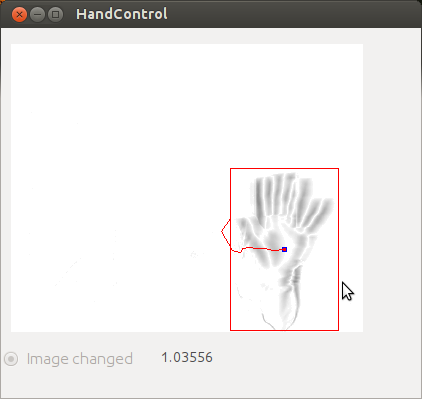
\includegraphics[width=0.55\textwidth]{images/Screenshot_ruka}
    \caption{Správne rozpoznaná ruka a jej predchádzajúca trajektória }
\end{figure}

\begin{figure}[h]
    \centering
    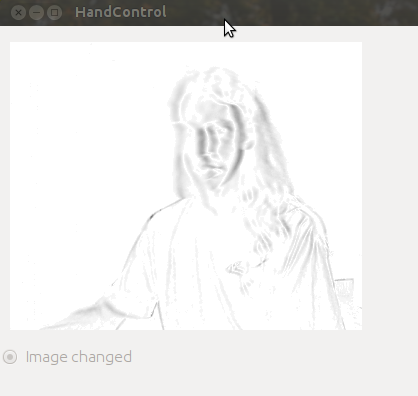
\includegraphics[width=0.55\textwidth]{images/Screenshot_clovek}
    \caption{Správne rozpoznaný iný objekt}
\end{figure}

